% diagrams-Bd.tex
\begin{hcarentry}[updated]{diagrams}
\report{Brent Yorgey}%11/16
\status{active development}
\participants{many}
\makeheader

The diagrams framework provides an embedded domain-specific language
for declarative drawing.  The overall vision is for diagrams to become
a viable alternative to DSLs like MetaPost or Asymptote, but with the
advantages of being \emph{declarative}---describing what to draw, not
how to draw it---and \emph{embedded}---putting the entire power of
Haskell (and Hackage) at the service of diagram creation.  There is
always more to be done, but diagrams is already quite fully-featured,
with a comprehensive user manual and a growing set of tutorials, a
large collection of primitive shapes and attributes, many different
modes of composition, paths, cubic splines, images, text, arbitrary
monoidal annotations, named subdiagrams, and more.

%**<img width=400 src="./3d-cubes.jpg">
%*ignore
\begin{center}
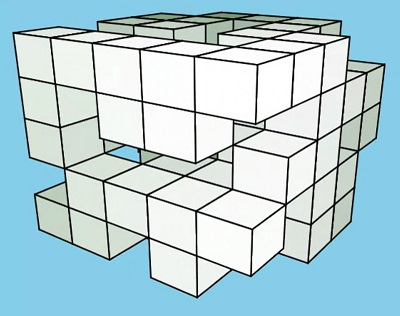
\includegraphics[width=0.47\textwidth]{html/3d-cubes.jpg}
\end{center}
%*endignore

\subsubsection*{What's new}

Diagrams 1.4 was released at the end of October, and mostly just adds
new features, such as:

\begin{compactitem}
\item B-spline support, and B-spline to cubic Bezier conversion
\item Boolean operations on paths, such as union and intersection
\item CSG support for 3D diagrams
\item New techniques and tools for drawing 2D projections of 3D
  diagrams, illustrated above
\item Constraint-based layout
\end{compactitem}

%**<img width=350 src="./kaleidoscope.jpg">
%*ignore
\begin{center}
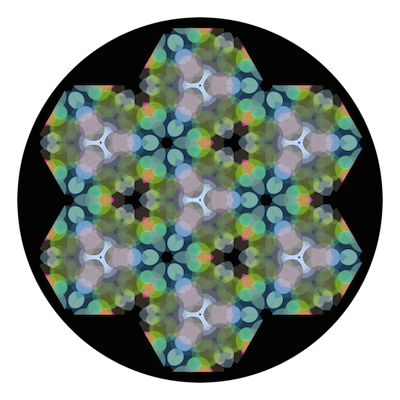
\includegraphics[width=0.45\textwidth]{html/kaleidoscope.jpg}
\end{center}
%*endignore

\subsubsection*{Contributing}

There is plenty of exciting work to be done; new contributors are
welcome!  Diagrams has developed an encouraging, responsive, and fun
developer community, and makes for a great opportunity to learn and
hack on some ``real-world'' Haskell code.  Because of its size,
generality, and enthusiastic embrace of advanced type system features,
diagrams can be intimidating to would-be users and contributors;
however, we are actively working on new documentation and resources to
help combat this.  For more information on ways to contribute and how
to get started, see the Contributing page on the diagrams wiki:
\url{http://haskell.org/haskellwiki/Diagrams/Contributing}, or come
hang out in the \texttt{\#diagrams} IRC channel on freenode.

%**<img width=400 src="./arrows.jpg">
%*ignore
\begin{center}
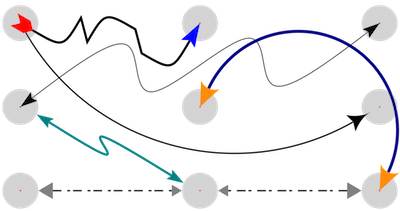
\includegraphics[width=0.47\textwidth]{html/arrows.jpg}
\end{center}
%*endignore

\FurtherReading
\begin{compactitem}
\item \url{http://projects.haskell.org/diagrams}
\item \url{http://projects.haskell.org/diagrams/gallery.html}
\item \url{http://haskell.org/haskellwiki/Diagrams}
\item \url{http://github.com/diagrams}
\item \url{http://ozark.hendrix.edu/~yorgey/pub/monoid-pearl.pdf}
\item \url{http://www.youtube.com/watch?v=X-8NCkD2vOw}
\end{compactitem}
\end{hcarentry}
